\chapter{Software Implementation}
\label{chap4}

The details of implementation will be described in this chapter. The modules will be explained in the chronological order in which they were implemented.

\section{Project Building}

For arbitrary Graphics API programming, setting up the development environment is complex and time-consuming and error-prone. As discussed in \ref{premake} and \ref{premake2} the Visual Studio solution will be generated through Premake5. Premake5 only contains an execute program; the configuration needs to be written to Lua scripts. The syntax of premake scripts is fixed; it should contain the basic configurations of the project, including languages, names, platforms, source code formats and others. Premake has many valuable tokens for setting the relative directories for input and output, the different settings for platforms are distinguished through the filters. Besides, in this project, many external libraries (e.g. GLFW, GLM, ImGui) need to be contained and compiled with the source file, premake can be used to set the libraries as StaticLib projects and linked to the main project, which will keep the source code of main project independent with the libraries. 

\hspace*{\fill}

After editing the scripts, the solution can be generated by Premake correctly as shown in figure \ref{impl:premake} and \ref{impl:solution}.

\begin{figure}[htbp]
    \centering
    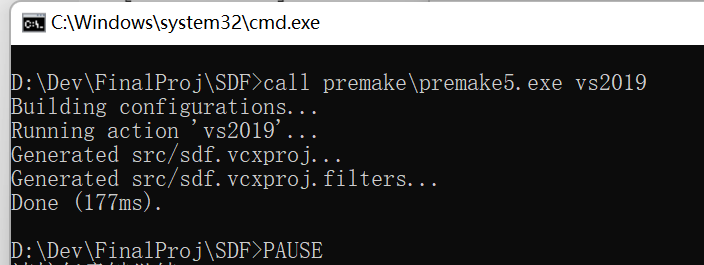
\includegraphics[width=13cm]{Images/Chap4/project.png}
    \caption{Generate Project Solution by Premake}
    \label{impl:premake}
\end{figure}

\clearpage

\begin{figure}[htbp]
    \centering
    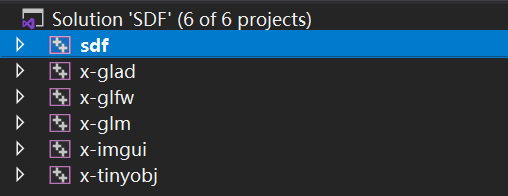
\includegraphics[width=12cm]{Images/Chap4/solution.png}
    \caption{The VS2019 Solution of this project}
    \label{impl:solution}
\end{figure}

The script code for whole solution and external libraries can be seen in Appendix \ref{ap:premake}.

\section{Basic Visualization Application}

In the first stage, a basic visualization application must be created to test whether the development environment is running properly. The modules will be implemented according to the design of the rendering process, which has been discussed in \ref{ds:visual}.

\paragraph{Shader Class}

The Shader class must load and compile shader files according to their type, and several overloaded constructors are implemented for the vertex shader, fragment shader and other options. The class invoke several gl functions for binding and compiling.

The code of constructor and creating function are shown in Listings \ref{lst:shadercons} and \ref{lst:shadercreate}.

\begin{lstlisting}[language=C++, label={lst:shadercons}, caption = Constructor of vertex and fragment shader]
    SHADER::SHADER(const char* vertex_path, const char* fragment_path)
{
    GLuint vertex_shader = create_shader(vertex_path, ShaderType::Vertex);
    GLuint fragment_shader = create_shader(fragment_path, ShaderType::Fragment);

    id = GL( glCreateProgram());
    GL( glAttachShader(id, vertex_shader) );
    GL( glAttachShader(id, fragment_shader) );
    GL( glLinkProgram(id) );

    if (check_shader_errors(id, ShaderType::Program)) exit(1);

    GL( glDeleteShader(vertex_shader) );
    GL( glDeleteShader(fragment_shader) );
}
\end{lstlisting}

\hspace*{\fill}
\hspace*{\fill}

\begin{lstlisting}[language=C++, label={lst:shadercreate}, caption = Function of creating shader]
GLuint SHADER::create_shader(const char* path, ShaderType type) const
{
    std::stringstream shader_stream;
    shader_stream << file.rdbuf();
    file.close();
    const std::string& shader_source = shader_stream.str();
    const char* shader_source_c_str = shader_source.c_str();
    GLenum shader_type = GL_VERTEX_SHADER;
    switch (type)
    {
        case ShaderType::Fragment:
            shader_type = GL_FRAGMENT_SHADER;
            break;
        case ShaderType::Compute:
            shader_type = GL_COMPUTE_SHADER;
            break;
    }
    GLuint SHADER = GL( glCreateShader(shader_type) );
    GL( glShaderSource(SHADER, 1, &shader_source_c_str, 0) );
    GL( glCompileShader(SHADER) );
    if (check_shader_errors(SHADER, type)) 
        return GLuint(-1);
    return SHADER;
}
\end{lstlisting}

\paragraph{Camera}

The camera class is implemented as a sphere orbit camera; the camera's position will rotate on a sphere orbit outside the object, whose centre is the centre of the object. There are several parameters needed to store the transformation matrices and scales. The project directly used the data structure provided by the GLM library for storing and computing. As for the operation mode, hold the right or middle mouse button, drag to move the camera, and use the mouse wheel to zoom. 

\hspace*{\fill}

The camera matrix transformation is implemented in the step() function and updated per frame, whose implementation can be seen in Listing \ref{lst:camerastep}.

\clearpage

\begin{lstlisting}[language=C++, label={lst:camerastep}, caption = Function of matrix transformation]
    void step( float elapse, const mouse_t &mouse ) {
    const glm::vec2& mouseD = mouse.mouseD;
    const glm::vec2& wheelD = mouse.wheelD;
    glm::vec3 delta( mouseD.x , -mouseD.y, 0 );
    // right button + mouse :rotation
    if ( mouse.button_stats[2] ) {
        orbit.x = constrain360( orbit.x + delta.y * rot_scaler );
        orbit.y = constrain360( orbit.y + delta.x * rot_scaler );
    }
    zoom = glm::clamp( -wheelD.y * zoom_scaler + _zoom, 10.f, 1000.f  );
    glm::mat4  rotation = glm::mat4( glm::rotate( glm::radians( _orbit.y ), Y ) ) * glm::mat4( glm::rotate( glm::radians( _orbit.x ), X ) )  ;
    if ( mouse.button_stats[1] ) {
        target += glm::mat3(rotation) * delta * pen_scaler ;
    }
    world = glm::translate( _target ) *  rotation * glm::translate( glm::vec3(0.f,0.f, _zoom) ) ; 
    view = glm::inverse( _world);
    proj = glm::perspective( glm::radians(_fov), _aspect, _near, _far );
    view_proj = _proj * _view;
}
\end{lstlisting}

\paragraph{GLFW Window}

An application window is necessary for rendering the GUI and models. As discussed in \ref{ds:rendering}, this project uses the GLFW library to create a rendering application. In this stage, a simple shader is used to test if the window is running correctly. A GLFW window should be instantiated to achieve the target and set the compulsory attributes, then get the user input data to control the camera. The step() function is invoked in the rendering loop function; frame time and the status of the mouse are stored in an object and passed to the Camera class for matrix computation. Listing \ref{lst:glfwinit} and \ref{lst:glfwrun} shows the code of GLFW window instantiation and rendering.

\begin{lstlisting}[language=C++, label={lst:glfwinit}, caption = GLFW window instantiation]
    GLFWwindow* window = nullptr ;
    glfwWindowHint(GLFW_OPENGL_DEBUG_CONTEXT, GL_TRUE); 
    // GL 4.5 
    glfwWindowHint(GLFW_CONTEXT_VERSION_MAJOR, 4);
    glfwWindowHint(GLFW_CONTEXT_VERSION_MINOR, 5);
    glfwWindowHint(GLFW_OPENGL_PROFILE, GLFW_OPENGL_CORE_PROFILE);
    glfwWindowHint(GLFW_OPENGL_FORWARD_COMPAT, GL_TRUE);
    // Create window with graphics context
    window = glfwCreateWindow(1280, 720, "SDF", NULL, NULL);
    if (!window)   exit(1);
\end{lstlisting}

\clearpage

\begin{lstlisting}[language=C++, label={lst:glfwrun}, caption = Rendering loop implementation]
    while (!glfwWindowShouldClose(window)) {
        // Camera update
        this->mouse.wheelD = {0,0};
        this->mouse.mouseD = {0,0};
        glfwPollEvents();
        float current = glfwGetTime();
        delta = current - last;
        accum += delta;
        last = current; 
        camera.step( delta, mouse );
        // Scene render
        glfwGetFramebufferSize(window, &screen_size.x, &screen_size.y);
        if (screen_size.x!=0 && screen_size.y!=0 ) {
            glViewport(0, 0, screen_size.x, screen_size.y);
            glClear(GL_COLOR_BUFFER_BIT | GL_DEPTH_BUFFER_BIT);

            app_draw_scene( delta );
            gui_draw(clear_color);
            glfwSwapBuffers(window);
        }
    }
\end{lstlisting}

\paragraph{Scene}

The infinite grid scene will be implemented through the vertex shader and fragment shader as the method introduced by Marie \cite{scene}. The GLSL source code can be seen in the Appendix \ref{ap:scene}. The shaders are loaded to the application and compiled by the shader class to create a shader program object, then bind the object as a part of the rendering state.

\paragraph{Graphical User Interface}

The GUI is implemented through the Dear ImGui library, and the GUI panel is created by invoking the functions of the library. First, it needs to be initialized to set the window pointer for the GUI panel. Then members of the GUI will be created. For example, ImGui::CollapsingHeader() function can be used to create an independent area on the panel, and ImGui::Checkbox() can be used to create a checkbox object on the panel.

\hspace*{\fill}

Listing \ref{lst:guimpl} shows the GUI implementation code.

\begin{lstlisting}[language=C++, label={lst:guimpl}, caption = ImGui panel implementation]
    // Setup Platform/Renderer backends
    ImGui_ImplGlfw_InitForOpenGL(window, true);
    ImGui::Begin( "Panel", 0 );
    // Visibility of model
    if (ImGui::CollapsingHeader("Visibility", ImGuiTreeNodeFlags_DefaultOpen ))
    {
        static bool shows[5];
        ImGui::Checkbox("Grid", &show_grids);
        ImGui::Checkbox("Polygon", &show_polygon );
        ImGui::Checkbox("Coloured Model", &show_color );

        ImGui::Checkbox("SDF", &show_iso );
        ImGui::Checkbox("RT Approximation", &show_sdf);
    }
    // Camera Status
    if (ImGui::CollapsingHeader("Cemera", ImGuiTreeNodeFlags_DefaultOpen)) {
        ImGui::LabelText( "Orbit", "%2.0f %2.0f" , camera._orbit.x, camera._orbit.y );
        ImGui::LabelText( "Target", "%2.0f %2.0f %2.0f", camera._target.x, camera._target.y ,camera._target.z );
        ImGui::LabelText( "Zoom", "%2.0f", camera._zoom  );
    }
    ImGui::End();
    // Rendering
    ImGui::Render();
    ImGui_ImplOpenGL3_RenderDrawData(ImGui::GetDrawData());
\end{lstlisting}

Once all of the processes have been completed, a window that renders an infinity grid scene and GUI panel can be seen on the screen as figure \ref{impl:gui}.

\begin{figure}[htbp]
    \centering
    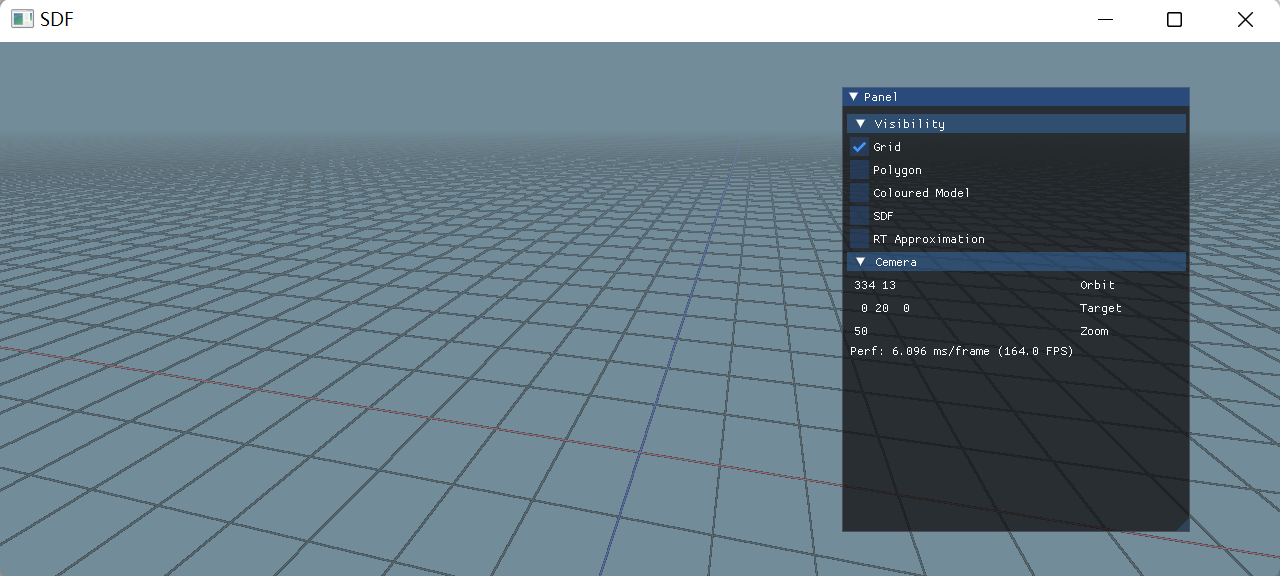
\includegraphics[width=16cm]{Images/Chap4/GUI.png}
    \caption{The basic infinity grid scene and GUI implementation}
    \label{impl:gui}
\end{figure}

\clearpage

\section{Model Rendering}

\paragraph{Model Class}

To load a triangular mesh, the tiniobjloader is used to get the vertices and face indices information. The vertices and the face indices are used to create triangle primitives for rendering and the signed distance function calculation. Several gl functions are used in the primitive creating stage.

The pseudocode of the load model is shown in Listing \ref{lst:modeload}.

\begin{lstlisting}[language=C++, label={lst:modeload}, caption = Pseudocode of model loading]
    load( obj_file ) {
    //Create empty containers
    tinyobj::attrib_t attrib;
    std::vector<tinyobj::shape_t> shapes;
    tinyobj::LoadObj(&attrib, &shapes, obj_file) // Load obj file
    // Clear the vectors
    vertices.clear();
    indices.clear();
    for (loop shape : shapes) { // Loop meshes to get vertices
        for (loop index : shape.mesh.indices) {
        vertex.pos = {
            attrib.vertices[3 * index.vertex_index + 0],
            attrib.vertices[3 * index.vertex_index + 1],
            attrib.vertices[3 * index.vertex_index + 2]    };
        vertices.push_back(vertex);     }   }   }
    triangles.resize( _indices.size()/3 );
    for ( size_t i=0;i<_triangles.size(); ++i) {
        auto i0 = _indices[i*3+0];
        auto i1 = _indices[i*3+1];
        auto i2 = _indices[i*3+2];
        triangles[i]._init( vertices[i0],vertices[i1],vertices[i2]); }
    make_primitive( vertices, indices );    }  
\end{lstlisting}

The code for making primitives are illustrated through Listing \ref{lst:modelprim}.

\begin{lstlisting}[language=C++, label={lst:modelprim}, caption = Function of creating triangular primitives]
void MODEL::make_primitive( const  vertex_t *Vdata, GLuint Vcount, 
        const uint32_t *Idata, GLuint Icount ) {
    _primitive.ibo_count = Icount;
    // Create VAO
    glGenVertexArrays(1, &_primitive.vao);
    glBindVertexArray( _primitive.vao);
    // create VBO
    glGenBuffers(1, &_primitive.vbo );
    glBindBuffer(GL_ARRAY_BUFFER, _primitive.vbo );
    // copy vertex attribs data to VBO
    GLuint vsize = sizeof(Vdata[0]) * Vcount;
    glBufferData(GL_ARRAY_BUFFER,  vsize, Vdata, GL_STATIC_DRAW);
    // Setup vertex attributes
    glVertexAttribPointer(0,3, GL_FLOAT, GL_FALSE, sizeof(Vdata[0]), 0); 
    glVertexAttribPointer(1,3, GL_FLOAT, GL_FALSE, sizeof(Vdata[0]),
        (GLvoid*) long( sizeof( Vdata[0].pos ) ));  
    glEnableVertexAttribArray(0);
    glEnableVertexAttribArray(1);        
    // Create index buffer
    glGenBuffers(1, & _primitive.ibo );
    glBindBuffer(GL_ELEMENT_ARRAY_BUFFER, _primitive.ibo );
    glBufferData(GL_ELEMENT_ARRAY_BUFFER, Icount * sizeof(Idata[0]) ,
        Idata , GL_STATIC_DRAW);  
    glBindBuffer(GL_ARRAY_BUFFER,0);
    glBindBuffer(GL_ELEMENT_ARRAY_BUFFER,0);
    glBindVertexArray(0);   }  
\end{lstlisting}

\paragraph{Rendering}

In the GUI implementation, two modes are set for model rendering, polygonal mode and coloured mode. Both can bind the same shaders, while the polygonal mode can be implemented by invoking the glPolygonMode(). The primitives of the model are set as triangles. Therefore, the draw mode should be set as GL\_TRIANGLES.

\hspace*{\fill}

Listing \ref{lst:modeldraw} shows the code of both modes.

\begin{lstlisting}[language=C++, label={lst:modeldraw}, caption = Function of creating triangular primitives]
    auto prim = &model._primitive; // Draw model primitives
    model_prog->bind(); // Bind shader
    // Setup transfrom
    model_prog->set_mat4( "MVP", glm::value_ptr( view_proj ) );
    prim->bind();
    if ( show_color ) { // Coloured draw mode
        model_prog->set_vec4( "COLOR", 0,0,0,0 );
        glDrawElements( GL_TRIANGLES , prim->ibo_count,
            GL_UNSIGNED_INT, (0) );
    }
    if ( show_polygon ) { // Polygonal draw mode
        glPolygonMode(GL_FRONT_AND_BACK, GL_LINE);
        model_prog->set_vec4( "COLOR", 1,1,1,1 );
        glDrawElements( GL_TRIANGLES , prim->ibo_count, 
            GL_UNSIGNED_INT, (0) );
        glPolygonMode(GL_FRONT_AND_BACK, GL_FILL);
    }
    prim->unbind();
    model_prog->unbind();
\end{lstlisting}

\clearpage

The result of both rendering modes can be seen in figure \ref{impl:modelrender}.


\begin{figure}[htbp]
    \centering
    \subfigure[Coloured Mode]{
        \begin{minipage}[b]{0.55\textwidth}
        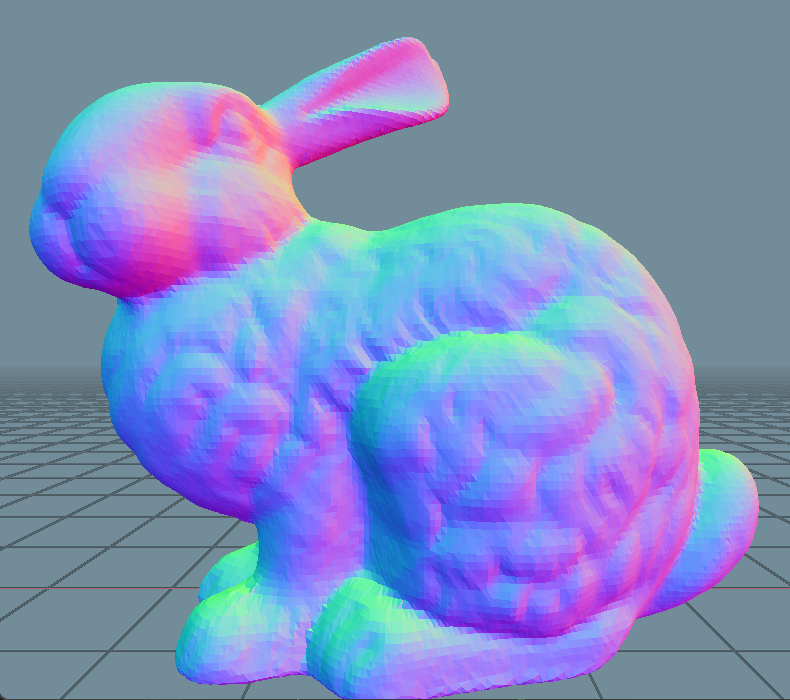
\includegraphics[width=1\textwidth]{Images/Chap4/colour.png}
        \end{minipage}
    }
    \subfigure[Polygonal Mode]{
        \begin{minipage}[b]{0.55\textwidth}
        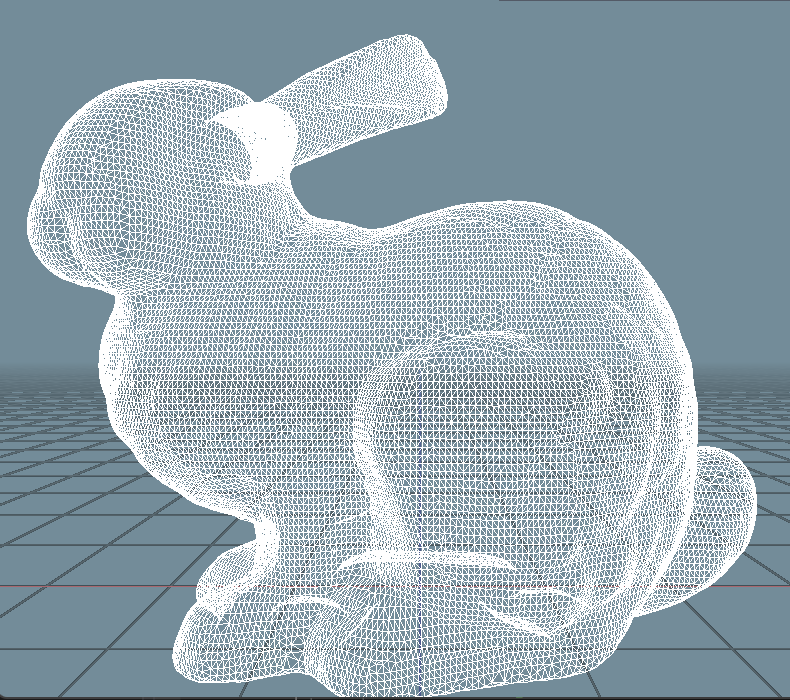
\includegraphics[width=1\textwidth]{Images/Chap4/polygon.png}
        \end{minipage}
    }
    \caption{The result of model rendering}
    \label{impl:modelrender}
\end{figure}

\section{Algorithm}

\subsection{KD-Tree}

To implement the KD-tree structure, the tree node needs to define a tree node class and then define the tree class as the derived class of the node. Since the primitives of a model are triangles, the triangle tree nodes need more data members to store their attributes like vertices and edges, while the tree class need children pointers and the split axis. Therefore, the node class is defined as an abstract class inherited by the triangle and tree class to add more variables.

\begin{breakablealgorithm}
    \caption{KD-Tree Building}
    \label{ds:kdbuild}
    \begin{algorithmic}

        \Require objects
        \State Building bounding box
        \State Set split Axis
        \Statex
        \State split bounding box
        \For{each objects i}
        \If{object[i].Bbox.center < objects.Bbox.middle}\\
                \Comment{Bbox is the bounding box of current object}
        
        \State Insert to left tree
        \Else
        \State Insert to right tree
        \EndIf
        \EndFor
        \State newBbox = left.Bbox + right.Bbox
    \end{algorithmic}
\end{breakablealgorithm}

\subsection{Ray Intersection}

There are three situations of ray-model intersection problem. If the ray start point is inside the bounding box, then the intersection status is set as true. If the ray intersects with any axis, the return value is also set as true. Otherwise, there is no intersection.

\hspace*{\fill}

The pseudocode is provided in Algorithm \ref{alg:bboxinter} below.

\begin{algorithm}[H]
    \caption{Bounding Box Intersection}
    \label{alg:bboxinter}
    \begin{algorithmic}
        \If{ray origin is inside of Bbox}
        \State return true
        \ElsIf{ray intersect with bounding box}
        \State return true
        \Else
        \State return false
        \EndIf
    \end{algorithmic}
\end{algorithm}

After completing the judgement of the intersection between ray and bounding box, the application uses the algorithm of Tomas Akenine-M{\"o}ller and Ben Trumbore \cite{AkenineMller2005FastMS} to calculate the distance function and sign function. Then the signed distance value will be stored in the intersection object for distance value comparison.

\hspace*{\fill}

The pseudocode is provided in Algorithm \ref{alg:trinter}. The definition of variables in Algorithm \ref{alg:trinter} will follow the definitions of \cite{AkenineMller2005FastMS}, which can be double reviewed in Section \ref{br:dfc}.

\begin{breakablealgorithm}
    \caption{Triangle Intersection}
    \label{alg:trinter}
    \begin{algorithmic}
        \Require EPSILON    \Comment{minimal interval from \cite{AkenineMller2005FastMS}}
        \State ray r  \Comment{denote origin as O, direction as D}
        \State triangle vertices $ V_{0}, V_{1} $ and $ V_{2}$
        \State triangle edges $ E_{1} $ and $ E_{2} $
        \State previous intersection inter\Comment{default as infinity}
        \Statex
        \State $ P = D\times E_{2} $
        \State $ determinant = E_{1} \cdot P $    \Comment{wiil be denoted as det for short}
        \State $ T = O - V_{0} $
        \Statex
        \If{det < EPSILON}
        \State return false
        \EndIf
        \Statex
        \State $ u = T \cdot P $
        \If{u < 0 or u > det}
        \State return false
        \EndIf
        \Statex
        \State $ Q = T \times E_{1} $
        \State $ v = D \cdot Q $
        \Statex
        \If{$ v < 0 $ or $ u + v > det $}
        \State return false
        \EndIf
        \Statex
        \State $  t = Q \cdot E_{2} $
        \State $  InvDet = 1{\div} det $
        \State $  t = t * InvDet $
        \If{$ t < inter.t $ and $ t > EPSILON $}
        \State update inter variable
        \State return true
        \Else \hspace{2pt} return false
        \EndIf
    \end{algorithmic}
\end{breakablealgorithm}

\subsection{Signed Distance Field Generation}

Finally, the ray intersection algorithm is applied to the field generation function. As discussed in the \ref{br:algorithm2}, each sampling voxels generate a number of rays from its centre to test and compute the distance. The first step is to loop a single voxel's ray group and get its minimal distance; the Algorithm \ref{alg:trinter} is used for single ray intersection judgement. Then test if the ray start point is inside the model or if the model has a hole to determine the sign of this voxel. Finally, record the signed distance value and repeat the process to each voxel. The ray intersection computation algorithm is implemented in the KD-tree structure for pruning.

\hspace*{\fill}

Listing \ref{lst:sampleRays} provides the code of sample rays generation.

\begin{lstlisting}[language=C++, label={lst:sampleRays}, caption = Function of generating sample rays for voxels]
    vector<vec3> sampleRays;
    sampleRays.clear();
    vec3 sum(0);
    float phiOffset = PI / phiSteps * 0.5f;
    for (int phiStep = 0; phiStep < phiSteps; phiStep++)
    {
        float phi = -PI / 2.f + (PI * phiStep) / phiSteps + phiOffset;
        for (int thetaStep = 0; thetaStep < thetaSteps; thetaStep++)
        {
            float theta = (PI * 2.f * thetaStep) / thetaSteps;
            vec3 direction(cosf(theta), sinf(theta), sinf(phi));
            sum += normalize(direction);
            sampleRays.push_back(normalize(direction));
        }
    }
\end{lstlisting}

The pseudocode of the field generation algorithm is shown in Algorithm \ref{alg:sdfgen}:

\begin{breakablealgorithm}
    \caption{SDF Generation}
    \label{alg:sdfgen}
    \begin{algorithmic}
        \Require mesh, dimensions, sampleRays
        \Statex
        \State Bbox = mesh.bbox     \Comment{The bounding box of the mesh}
        \State d = dimensions
        \State hit = 0
        \State hitBack = 0
        \Statex
        \For{each point p(x,y,z) in Bbox}
            \State minDistance = $ \infty $

            \For{each ray in sampleRays}
            \If{ray intersect with model}
                \State hit++
                \If{ray intersect with backside}
                \State hitBack++
                \EndIf
                \If{currentDistance < minDistance}
                \State minDistance = currentDistance
                \EndIf
            \EndIf
            \EndFor

            \If{Over half of rays hit backside}
            \State The ray origin inside mesh
            \State sign is negative
            \EndIf

            \If{The meshes has hole}
            \State The ray origin inside mesh
            \State sign is negative
            \EndIf
        \State Distance at p(x,y,z) = minDistance
        \EndFor
    \end{algorithmic}
\end{breakablealgorithm}

The asynchronous multi-threading strategy is also applied to reduce the generation time. The voxels are divided into many groups, and each group will run the generation function in parallel. The method is implemented by using the std::async() function. 

\hspace*{\fill}

Listing \ref{lst:async} gives the code of multi-threading acceleration. The Algorithm \ref{alg:sdfgen} is implemented in function generate\_layer().

\begin{lstlisting}[language=C++, label={lst:async}, caption = Function of generating sample rays for voxels]
    auto future = std::async(std::launch::async, [&] {
        std::vector<int> zid (dfDimensions.z);
        std::iota (std::begin(zid), std::end(zid), 0); 
        
        std::for_each(
        std::execution::par,
        zid.begin(),
        zid.end(),
        [&](auto&& zIndex)
        {
            cout << "\tProcessing layer: " << zIndex << endl;
            generate_layer(model,sampleRays, 
                zIndex, _layer_progress[zIndex] );
        });
        return 0;
    });
\end{lstlisting}

\clearpage

\section{SDF output and debug}

The result of the signed distance field is stored in a text file since it is easy to be generated and validate. Operator << is overloaded to 
output the values. The implementation can be seen in Listing \ref{lst:sdfout}

\begin{lstlisting}[language=C++, label={lst:sdfout}, caption = SDF output function]
    ofstream &operator<<(ofstream &o, const SDF &data) {
        o << data._source << endl
        << data._grids.x << " " << data._grids.y << " " << data._grids.z << endl
        << data._resolution << endl;
        for (float f : data._voxels) //distance values
        {   o << f << endl;    }
        for (auto v : data._vertices) // sample voxels
        {   o << v.x << " " << v.y << " " << v.z << endl;   }
        return o;
    }
\end{lstlisting}

Some debug information needs to be shown on the interface, including generation time, triangle number and sampling resolutions. Therefore, the GUI panel implementation should add a new capsule area.

\hspace*{\fill}

The final GUI panel implementation is shown in figure \ref{impl:guidebug}.

\begin{figure}[htbp]
    \centering
    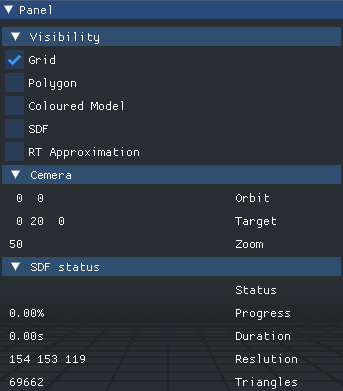
\includegraphics[width=9cm]{Images/Chap4/guidebug.png}
    \caption{GUI panel with debug info}
    \label{impl:guidebug}
\end{figure}

\clearpage

\section{SDF Visualization}
\label{impl:sdfvisual}

Finally, the result of the SDF calculation should be visualized. Two methods are implemented in this project, and the first one is using distance values to adjust the colour value; the volume of colour is changed according to the distance. The result is shown in figure \ref{impl:sdfiso},  the volume of green is set as the highest on the boundary of the model while the colour of inside voxels is visualized as red. The other one used ray tracing to approximate the model shape, which is shown in figure \ref{impl:sdfrt}.

\begin{figure}[htbp]
    \centering
    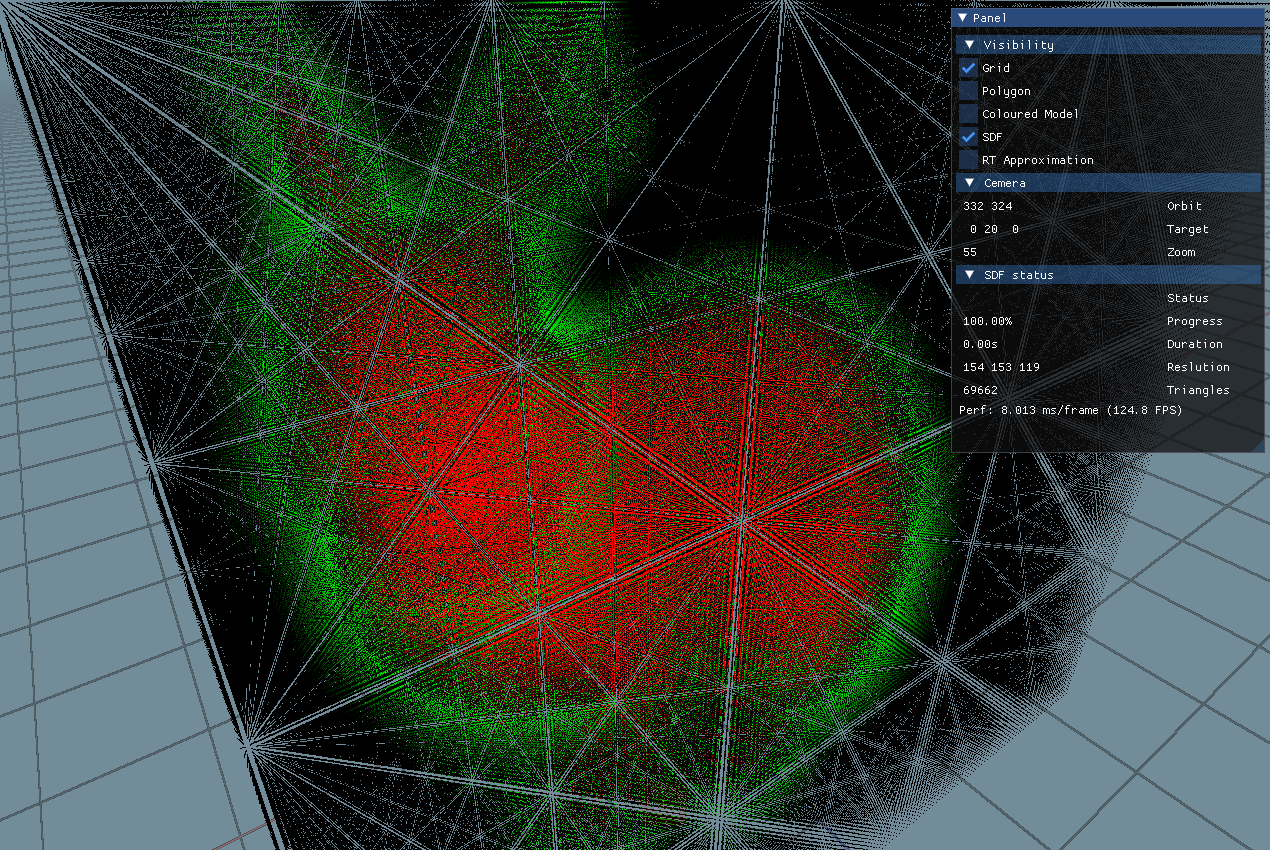
\includegraphics[width=12.6cm]{Images/Chap4/result.png}
    \caption{The colour volume mode of SDF visualization}
    \label{impl:sdfiso}
\end{figure}
\begin{figure}[htbp]
    \centering
    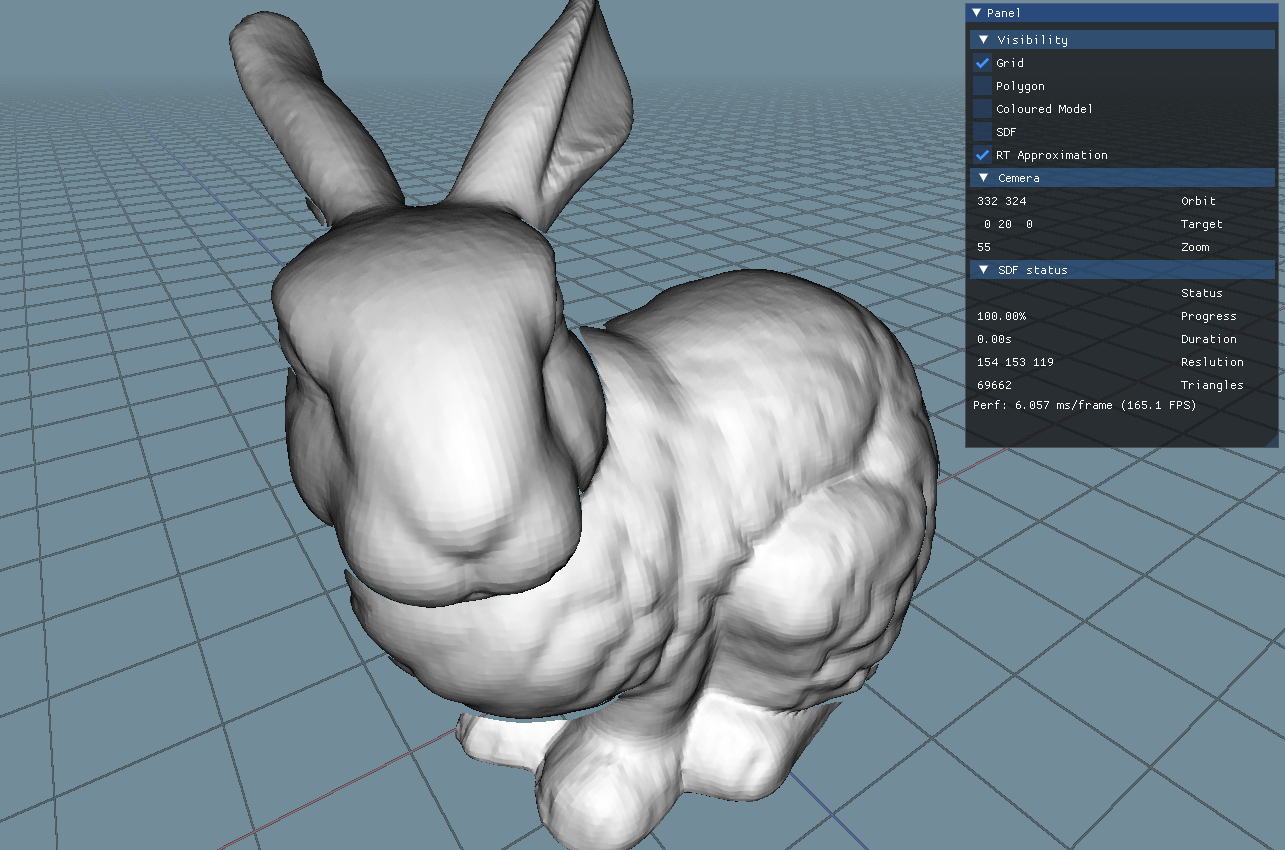
\includegraphics[width=12.6cm]{Images/Chap4/rta.png}
    \caption{The ray tracing mode of SDF visualization}
    \label{impl:sdfrt}
\end{figure}


\clearpage